% id: 118-74
% book: 100발100중 3-2 중간 · 01 3-2 중간(삼각비·삼각비의 활용·원과 직선·원주각·부록)
% section: 족집게 마무리 객관식 80선
% figure: crop:fig-118-74.png
% answer: ②
% answer_source: 답지(빠른정답)
% variant_level: 0 (원본 전사)
% 이 파일은 build.mjs 가 items.json 에서 만든다. 고칠 때는 items.json 을 고친다.
\smash{\raisebox{1.5mm}{\dmkichul{100발100중 3-2 중간 118쪽 74번}}}
\noindent\begin{minipage}[t]{0.58\linewidth}\vspace{0pt}\raggedright 그림과 같이 반지름의 길이가 $5\mkern3mu \mathrm{cm}$인 원~$\pt{O}$에 내접하는 $\triangle\pt{ABC}$에서 $\seg{BC}=6\mkern3mu \mathrm{cm}$일 때, $\cos A-\sin A$의 값은?\end{minipage}\hfill\begin{minipage}[t]{0.4\linewidth}\vspace{0pt}\centering 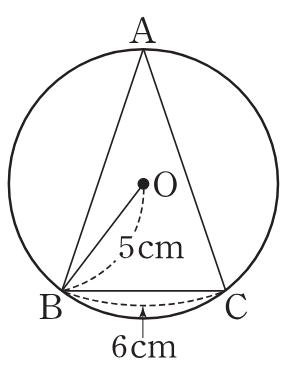
\includegraphics[width=68.6pt]{figures/fig-118-74.png}\end{minipage}\par
\begin{choicesii}{\rule[-3ex]{0pt}{8ex}$\dfrac{3}{4}$}{\rule[-3ex]{0pt}{8ex}$\dfrac{1}{5}$}{\rule[-3ex]{0pt}{8ex}$\dfrac{2}{5}$}{\rule[-3ex]{0pt}{8ex}$\dfrac{6}{5}$}{\rule[-3ex]{0pt}{8ex}$\dfrac{8}{5}$}\end{choicesii}
